\documentclass[conference]{IEEEtran}
\IEEEoverridecommandlockouts
% The preceding line is only needed to identify funding in the first footnote. If that is unneeded, please comment it out.
\usepackage{cite}
\usepackage{amsmath,amssymb,amsfonts}
\usepackage{algorithmic}
\usepackage{graphicx}
\usepackage{textcomp}
\usepackage{booktabs} 
\usepackage{float}      % enables the [H] placement specifier (exact placement)

% ---------- add these to the PREAMBLE (once) ----------
\usepackage{graphicx}   % already present in most IEEE templates
\usepackage{adjustbox}  % robust scaling
\usepackage{placeins}   % \FloatBarrier
\usepackage{siunitx}    % \num command for thousands separators
\usepackage{xcolor}
\def\BibTeX{{\rm B\kern-.05em{\sc i\kern-.025em b}\kern-.08em
    T\kern-.1667em\lower.7ex\hbox{E}\kern-.125emX}}
\begin{document}

\title{Grasping Emotion: A Vision-Based Study of Hand Movement and Feeling\\

\thanks{Identify applicable funding agency here. If none, delete this.}
}

\author{\IEEEauthorblockN{1\textsuperscript{st} Muhammed Almustafa}
\IEEEauthorblockA{\textit{Intelligent interactive systems Master's} \\
\textit{Bielefeld University}\\
Bielefeld,Germany \\
muhammed.almustafa@uni-bielefeld.de}
\and
\IEEEauthorblockN{2\textsuperscript{nd} Hakki Egemen Gülpinar}
\IEEEauthorblockA{\textit{Intelligent interactive systems Master's} \\
\textit{Bielefeld University}\\
Bielefeld,Germany \\
hakki.guelpinar@uni-bielefeld.de}
\and
\IEEEauthorblockN{3\textsuperscript{rd} Skryzhadlovska Anastasiia}
\IEEEauthorblockA{\textit{Intelligent interactive systems Master's} \\
\textit{Bielefeld University}\\
Bielefeld,Germany \\
anastasiia.skryzhadlovska@uni-bielefeld.de} 
}

\maketitle

\begin{abstract}
This study examines how emotional responses to different objects are reflected in hand movements during grasping. Using a smartphone camera with MediaPipe~\cite{mediapipe2019} and OpenCV~\cite{opencv2015}, we recorded hand kinematics from 20 participants as they naturally grasped five objects (cube, donut, pig toy, spider toy, plush). Half of the participants saw the objects before grasping; the other half did not.

After each grasp, participants completed a short emotional survey. We tested whether emotional responses influence grasp patterns and whether high-arousal emotions (e.g., fear) lead to faster, more forceful movements. The findings aim to reveal how emotion is expressed physically, using accessible tools for behavioral analysis.
\end{abstract}

\begin{IEEEkeywords}
component, formatting, style, styling, insert
\end{IEEEkeywords}

\section{Introduction}

The human hand is not merely a tool for physical interaction but also a subtle medium of emotional expression. Prior research has demonstrated that hand kinematics are not only responsive to object features such as weight, texture, and temperature but are also influenced by the emotional context in which interaction occurs. While foundational studies such as Lederman and Klatzky~\cite{b1} have shown that specific exploratory hand movements are associated with the extraction of object properties during haptic recognition, relatively few studies have examined how emotional valence modulates natural grasping behavior, particularly in real-life, unconstrained interactions.

Understanding the emotional component of grasping is crucial, especially in domains such as social robotics, affective computing, rehabilitation, and human-computer interaction, where affect-sensitive physical interaction is key~\cite{affective_haptics2023}. The interplay between emotion and action has been explored through facial expressions, vocal cues, and body posture, yet the nuanced expressiveness embedded in hand movements---especially during functional acts like grasping---remains under-investigated.

In this work, we aim to bridge this gap by studying how natural emotional responses to various objects are reflected in hand movement kinematics during grasping. We employed a non-intrusive method using a regular smartphone camera in combination with MediaPipe and OpenCV to track and analyze hand motion, allowing us to collect data in a naturalistic, accessible manner. Participants interacted with five different objects---a soft plush toy, a cube, a slime-like object, a fake spider, and a pig toy---each designed to evoke a distinct emotional response (e.g., comfort, neutrality, disgust, fear, amusement). Emotional feedback was collected through brief surveys after each grasp, enabling us to link movement patterns with subjective emotional states.

Our study is guided by two main research questions:

\begin{enumerate}
    \item Do different emotionally evocative objects produce significantly different hand kinematics during grasping?
    \item Does the emotional arousal level associated with an object influence the dynamism of grasping movements (e.g., speed, grip aperture, acceleration)?
\end{enumerate}

These questions are investigated under two experimental conditions: one in which participants were blindfolded (to isolate tactile perception) and one in which they viewed the object before grasping it (to include visual-emotional anticipation). This design allows us to evaluate both the conscious and subconscious influence of emotion on hand movement.

The remainder of the paper is structured as follows: In Section~\ref{sec:relatedwork}, we discuss related work on emotional expression in hand movement and haptic perception. Section~\ref{sec:methods} details our study design, including hypotheses, setup, data collection methods, and feature extraction. Section~\ref{sec:results} presents our results. In Section~\ref{sec:discussion}, we discuss the implications of our findings in the broader context of affective computing and embodied emotion. Finally, Section~\ref{sec:conclusion} concludes the paper with key insights and directions for future work.

\section{Related Work}
\label{sec:relatedwork}

Our study builds directly on the foundational work of Lederman and Klatzky~\cite{b1}, who demonstrated that hand movements during object exploration are highly structured and linked to specific perceptual goals. They introduced the concept of \textit{exploratory procedures} (EPs), which are stereotyped movement patterns---such as lateral motion, pressure, static contact, contour following, and enclosure---used intentionally to extract object properties like texture, hardness, temperature, shape, and weight. Through a series of experiments, they showed that participants consistently selected the most efficient and informative hand movements depending on the perceptual dimension they were exploring.

This framework has shaped our understanding of haptic exploration by emphasizing that hand movements are neither random nor solely biomechanical but are intentional and cognitively driven. In our study, we extend this idea into the domain of emotion-driven interaction by investigating whether affective responses also influence the kinematics of grasping. Specifically, we ask: can the emotional valence of an object---such as perceived pleasantness or threat---modulate the dynamics of hand movement during interaction?

Although Lederman and Klatzky focused on perceptual outcomes, recent studies suggest that emotion can similarly shape motor output. In particular, Esteves et al.~\cite{b2} demonstrated that participants' grasping movements varied systematically when interacting with emotionally charged objects. They found that grasping unpleasant stimuli resulted in lower peak velocities and longer movement times compared to pleasant or neutral stimuli, indicating that affective valence modulates temporal aspects of motor execution. This evidence supports the notion that emotional value, like perceptual goals, can influence the planning and unfolding of grasping movements.

To our knowledge, few studies have bridged these two domains—perception-based hand kinematics and affect-modulated motor behavior—within naturalistic grasping tasks. By integrating subjective emotional feedback with computer-vision-based motion tracking, our work seeks to fill this gap and offer a novel contribution to both haptic cognition and affective motor research.

\section{Methods}
\label{sec:methods}

This study investigated how natural emotional responses evoked by various objects are reflected in hand kinematics during grasping. We examined this under two experimental conditions: one where participants could visually perceive the objects while grasping, and another where visual information was withheld.

\subsection{Hypotheses}

Based on prior work linking emotion and motor behavior ~\cite{b1}~\cite{b2}, we proposed the following hypotheses:

    \textbf{Hypothesis 1:} Objects that evoke distinct emotional responses produce significantly different hand movement patterns (e.g., differences in velocity, interaction duration, grip strength).
    
    \textbf{Hypothesis 2:} Objects eliciting high-arousal emotions (e.g., fear, surprise) lead to faster and more forceful grasping movements than objects evoking low-arousal emotions (e.g., comfort, boredom).

\subsection{Procedure and Study Setup}

\subsubsection{Experimental Design}
We used a between-subjects design with two conditions:

    \textbf{Visual Condition:} Ten participants grasped objects placed openly on the table, allowing them to see each object fully before grasping and experience visual-emotional anticipation.
    
    \textbf{Non-Visual Condition: }For the other ten participants, the objects were positioned behind an opaque stand with a small opening, through which they inserted their hand to grasp the object without any visual information. This setup ensured that tactile perception was isolated from visual cues.

This design preserved the element of surprise and prevented participants from becoming familiar with the objects across both conditions. Each participant completed five trials (one grasp per object) within their assigned condition. Each trial/object was followed by a short emotional survey. Object sequence was randomized across participants to minimize order effects and bias.

\subsubsection{Stimuli}

Five objects (Fig.~\ref{fig:objects}) were selected to elicit distinct emotional responses:

\begin{itemize}
    \item Plain wooden cube (Neutrality)

    \item Soft plush toy ( Comfort/Happiness)

    \item Fake spider (Fear)

    \item Nutella donut (Disgust)

    \item Squeaky pig toy (Surprise)
\end{itemize}

\begin{figure}[H]
    \centering
    \includegraphics[width=\columnwidth]{objects.png}
    \caption{Stimuli used in the study}
    \label{fig:objects}
\end{figure}

\subsubsection{Setup and Recording}

Objects were placed around 35 cm from the participant on a marker-aligned table. Hand movements were recorded with an overhead smartphone camera (iPhone 14, 1080p at 60 fps) mounted 50 cm above the workspace (Fig.~\ref{fig:setup}).

\begin{figure}[H]
    \centering
    \includegraphics[width=\columnwidth]{setup.png}
    \caption{Schematic of the experimental setup}
    \label{fig:setup}
\end{figure}


\subsection{Participants and Data Collection}
\subsubsection{Participants}
Twenty young adults (ages 18–30) participated voluntarily, recruited from the student community at Bielefeld University. All were right-handed, with no self-reported neurological or psychiatric conditions. Participants provided informed consent before participation and were naive to the study hypotheses. The study followed ethical guidelines for research with human subjects.

\subsubsection{Data Collected}
Kinematic data were extracted from hand movements captured by the camera. We utilized MediaPipe~\cite{mediapipe2019} and OpenCV~\cite{opencv2015} to analyze hand motion and derive key kinematic measures. These included:

\begin{itemize}
    \item Average velocity (pixels/s) - hand center movement speed between frames
    \item Grasp duration (s) - time spent in each gesture category
    \item Hand openness ratio (0-1 scale) - fingertip extension normalized index
    \item Movement efficiency ratio - straight-line distance to actual path ratio
    \item Hand stability index - inverse coefficient of variation of velocity
    \item Grasping frequency (events/s) - number of grasping events per unit time
\end{itemize}

Subjective ratings were also recorded for each object to link emotional responses with kinematic features. Following each grasping trial, participants provided detailed feedback about their subjective experience through a survey, which was designed to capture both the qualitative nature of emotions experienced and quantitative aspects of their intensity.
Participants first identified their primary emotion from a list of the following options: \textit{Neutral, Happiness, Surprise, Fear, Disgust, Frustration, Sadness, Confusion, Boredom, Nervousness, or Other (with optional description).}
For each reported emotion, participants then rated:

\begin{itemize}
    \item Intensity (Low, Moderate, High)
    \item Comfort level during grasping (Very comfortable, Neutral, Uncomfortable)
    \item Familiarity with the object (Very familiar, Somewhat familiar, Not familiar at all)
\end{itemize}




% ------------------------------------------------------
% IV. RESULTS
% ------------------------------------------------------
\section{Results}
\label{sec:results}

\subsection{Participant Demographics and Data Overview}

Twenty participants (ages 18--30; 12 female, 8 male) completed the study, 
evenly distributed between \textsc{Visual} and \textsc{Non-Visual} conditions.
Hand-tracking analysis yielded \num{45634} grasping events across all 
participants and objects. The overall mean grasping frequency was 
$12.02 \pm 6.1\ \text{events/s}$, with an average hand detection time of 
$34.87\ \text{s}$ per trial.

\subsection{Object-Specific Kinematic Patterns}

Table~\ref{tab:summary} presents descriptive statistics for each object.
Notable differences emerged in grasping frequency, with the spider object 
eliciting the highest activity ($M = 18.09 \pm 8.00\ \text{events/s}$) 
and the donut the lowest ($M = 7.02 \pm 6.41\ \text{events/s}$).

\begin{table}[H]
\caption{Summary statistics for all participants. Values are mean $\pm$ SD.}
\label{tab:summary}
\centering
\footnotesize
\setlength{\tabcolsep}{3pt}
\begin{adjustbox}{max width=\columnwidth}
\begin{tabular}{lcccccc}
\toprule
\textbf{Object} &
\textbf{Avg.\ Detect.\ Time (s)} &
\textbf{Avg.\ Grasp Events} &
\textbf{Avg.\ Freq.\ (events/s)} &
\textbf{Avg.\ Vel.\ (px/frame)} &
\textbf{Max.\ Vel.\ (px/frame)} &
\textbf{Most Common Emotion} \\ \midrule
Box    & 29.5 & 345 & 10.3 & 1.6 & 2.4 & Neutral   \\
Donut  & 36.2 & 313 &  7.0 & 0.9 & 1.3 & Disgust   \\
Pig    & 35.2 & 387 &  9.5 & 2.5 & 3.5 & Happiness \\
Spider & 34.0 & 675 & 18.1 & 3.2 & 4.6 & Fear      \\
Toy    & 39.5 & 561 & 15.2 & 2.0 & 2.8 & Neutral   \\ \bottomrule
\end{tabular}
\end{adjustbox}
\end{table}

\subsection{Group Comparison: Visual vs. Non-Visual Conditions}

Participants in the \textsc{Visual} condition demonstrated a slightly higher mean 
grasping frequency ($M = 12.74 \pm 2.14\ \text{events/s}$) compared to 
the \textsc{Non-Visual} condition ($M = 11.31 \pm 5.65\ \text{events/s}$). 
However, a Mann-Whitney U test revealed this difference was not statistically 
significant ($U = 1398.0$, $p = 0.309$), indicating that visual preview did 
not significantly alter overall grasping behavior (Fig.~\ref{fig:grasping-groups}).

The effect size was small (Cohen's $d = 0.335$)~\cite{cohen1988}, suggesting minimal practical 
difference between conditions. Notably, the \textsc{Non-Visual} group showed 
greater variability in responses, particularly for emotionally charged objects.

\begin{figure}[!b]
    \centering
    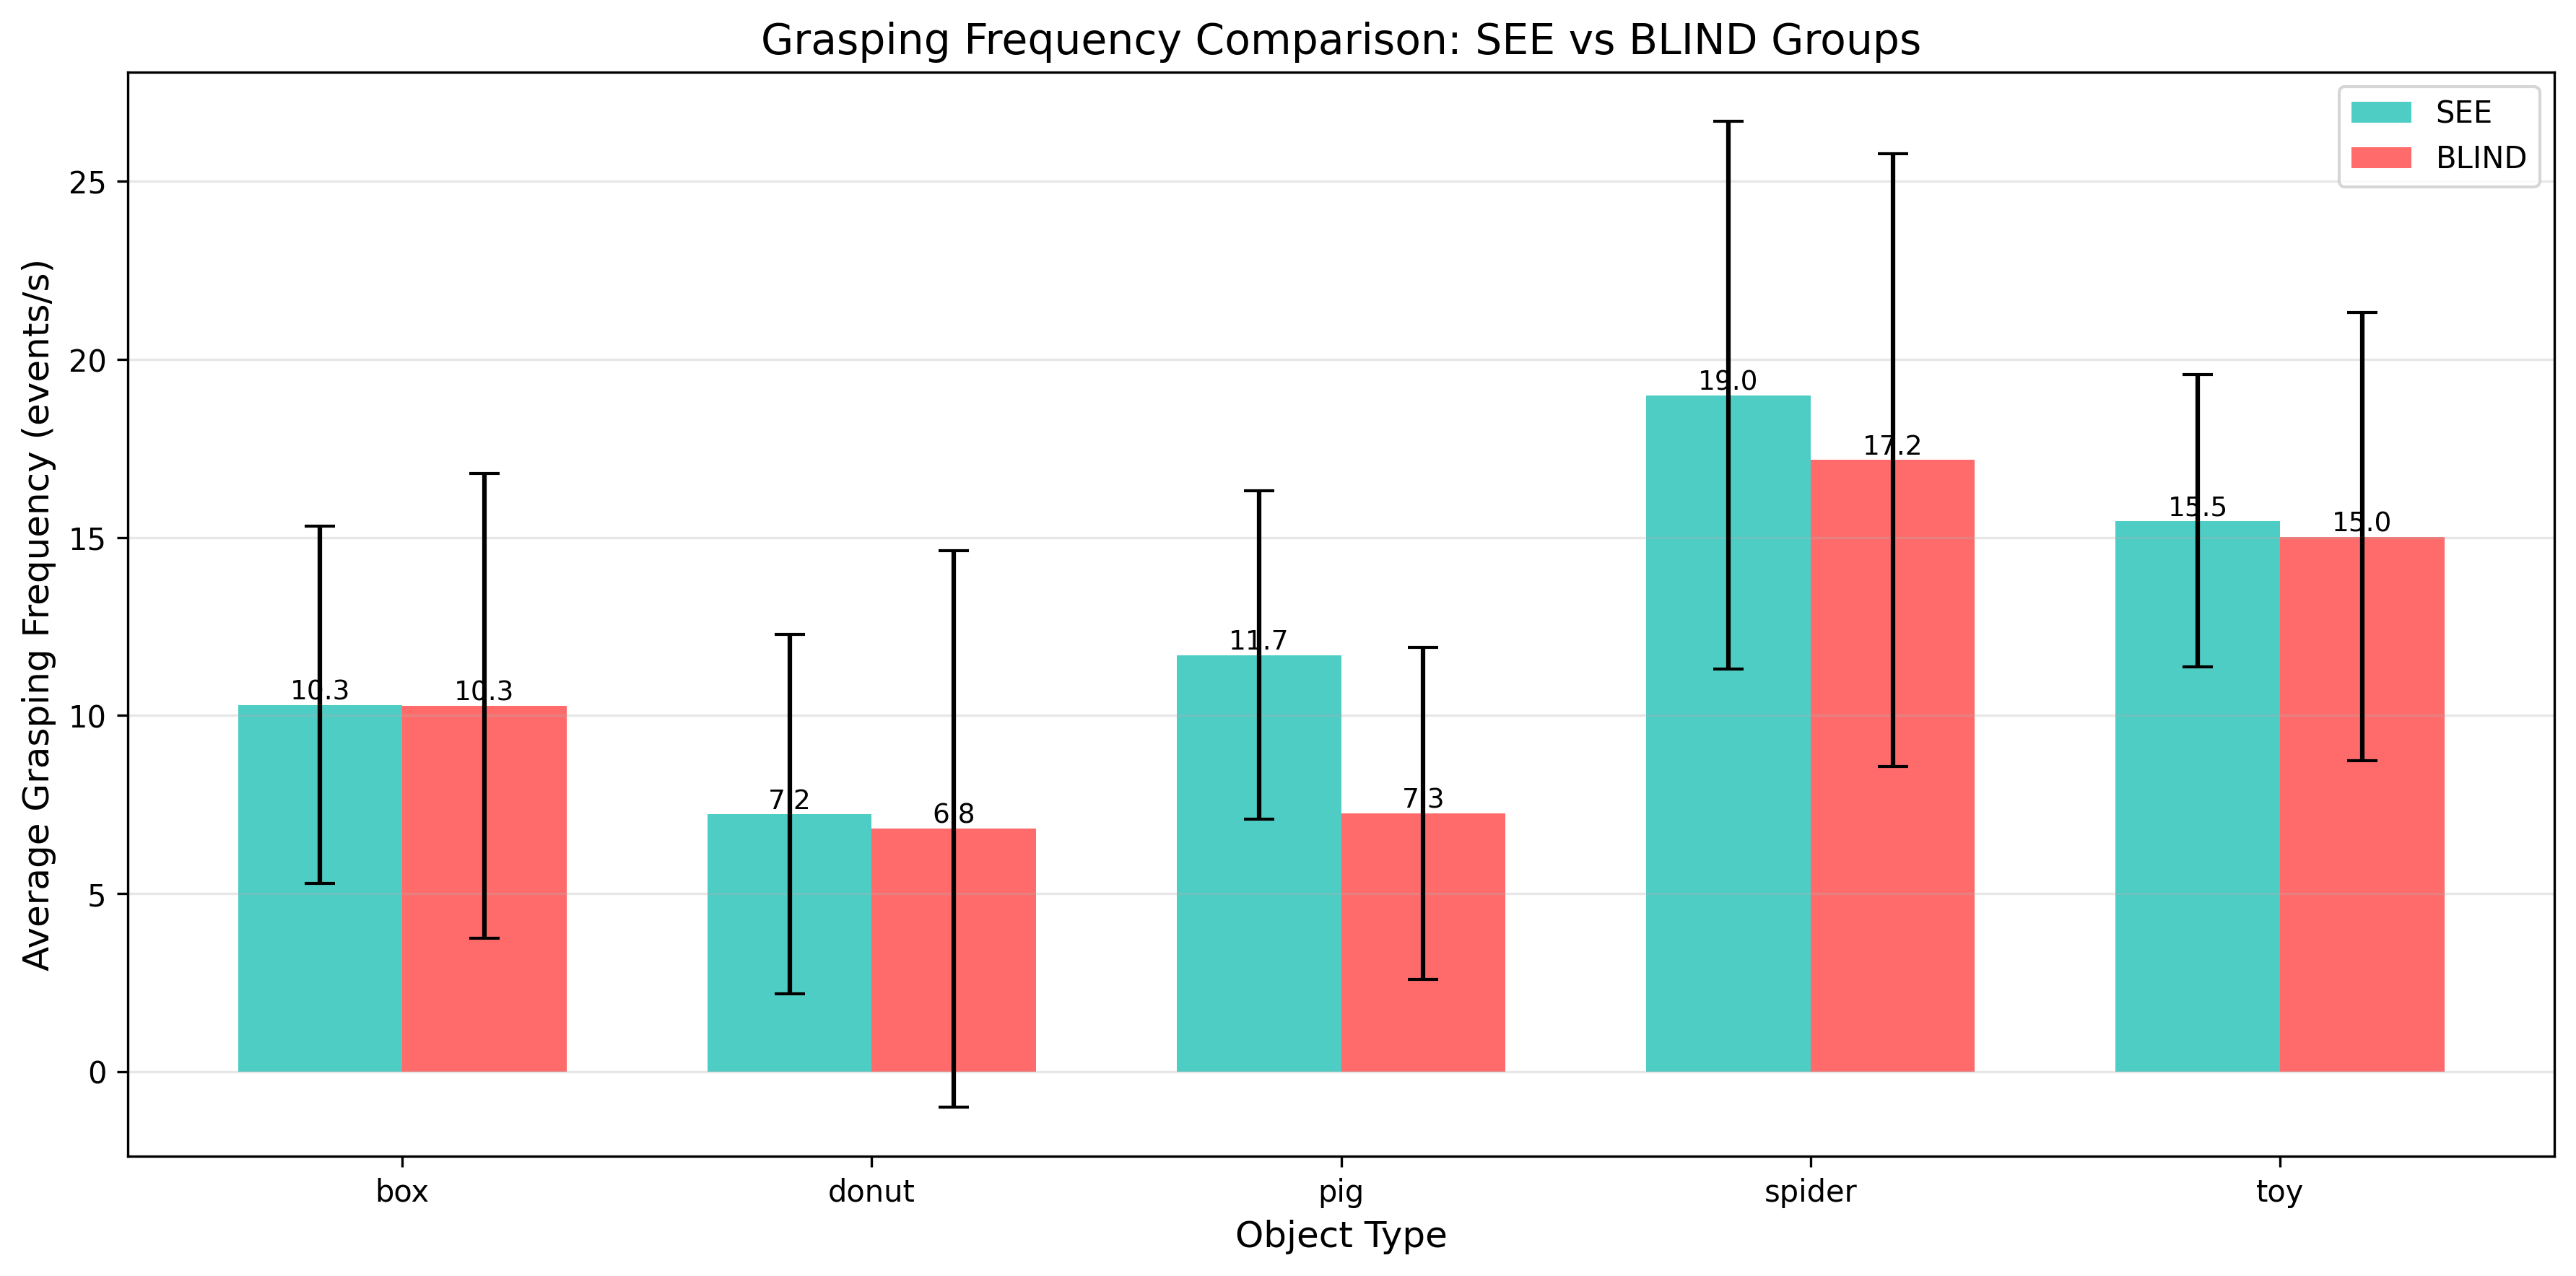
\includegraphics[width=\columnwidth]{group_main_analysis.png}
    \caption{Grasping frequency comparison between \textsc{Visual} and \textsc{Non-Visual} conditions by object type. Error bars represent standard error of the mean.}
    \label{fig:grasping-groups}
\end{figure}

\subsection{Movement Category Analysis}

Analysis of movement patterns revealed three distinct categories: grasping 
(active manipulation), holding (sustained contact), and other movements 
(exploratory or transitional). Figure~\ref{fig:movement-dist} shows the 
distribution across objects. The spider object elicited the highest 
proportion of active grasping movements (68.2\%), while neutral objects 
like the box showed more balanced distributions across categories.

\begin{figure}[!t]
    \centering
    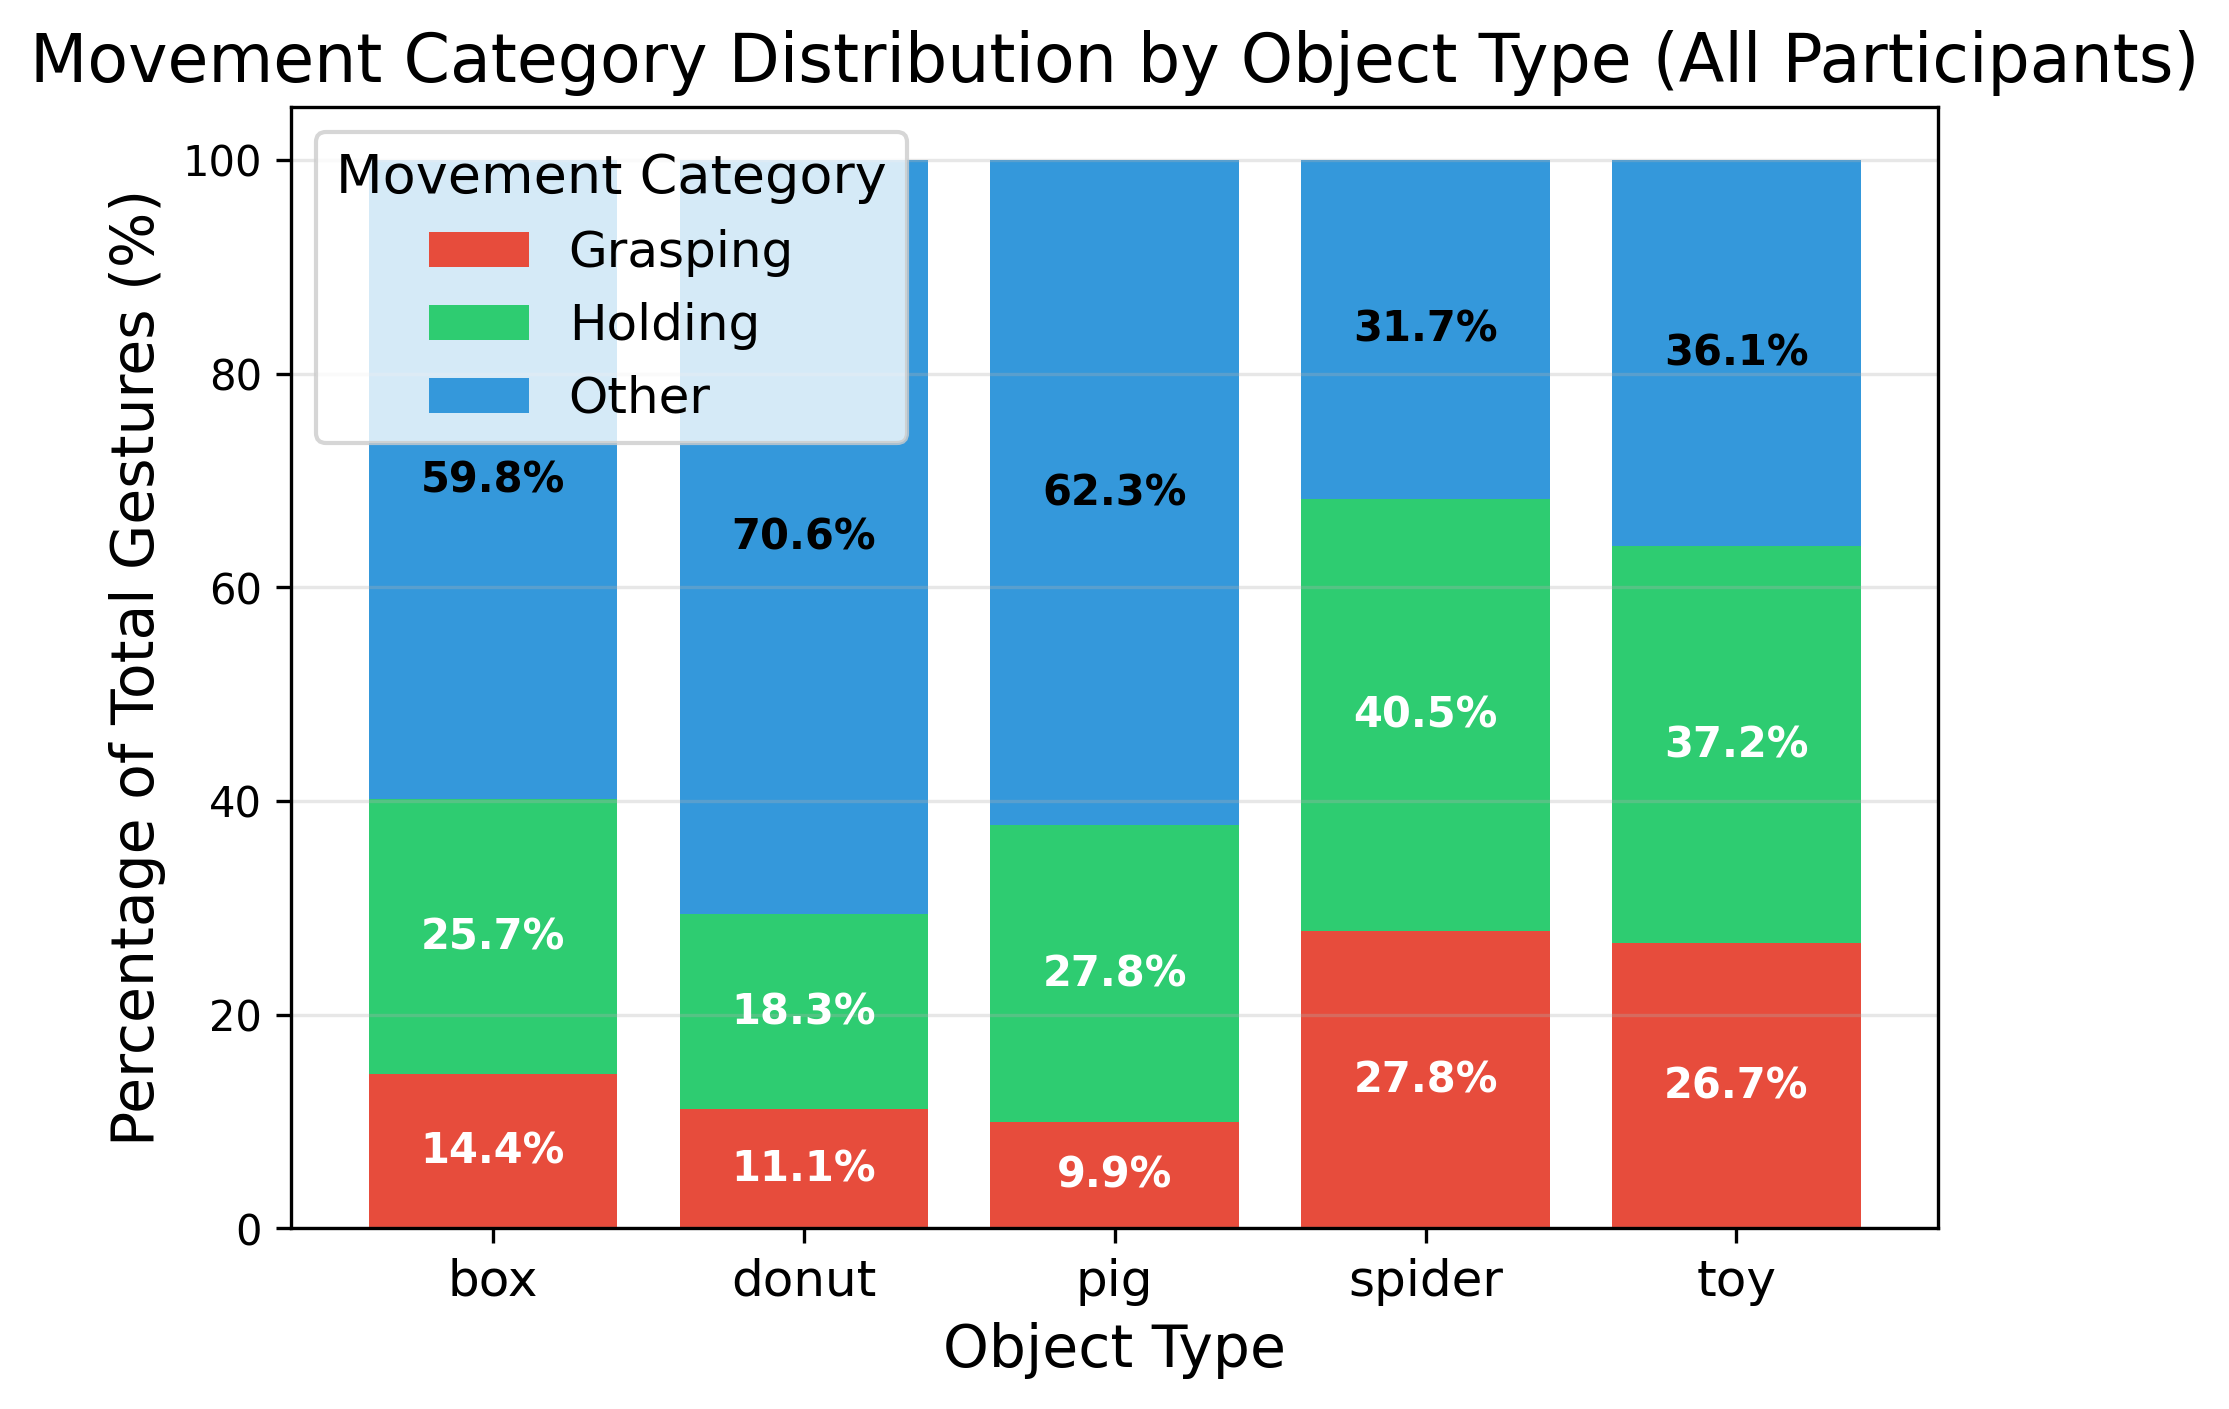
\includegraphics[width=\columnwidth]{avg_grasping_analysis.png}
    \caption{Distribution of movement categories by object type, showing percentage of grasping, holding, and other movements.}
    \label{fig:movement-dist}
\end{figure}

\subsection{Emotional Response Patterns}

Subjective emotional ratings aligned with object design intentions 
(Fig.~\ref{fig:emotion-dist}). The spider object primarily evoked fear 
responses (9 participants), while the donut elicited disgust (13 participants). 
Neutral emotions were most common overall (23 responses), followed by 
happiness (22 responses). High-arousal emotions (fear, surprise, disgust) 
were associated with increased grasping frequency, supporting \textbf{Hypothesis 2}.

\begin{figure}[!t]
    \centering
    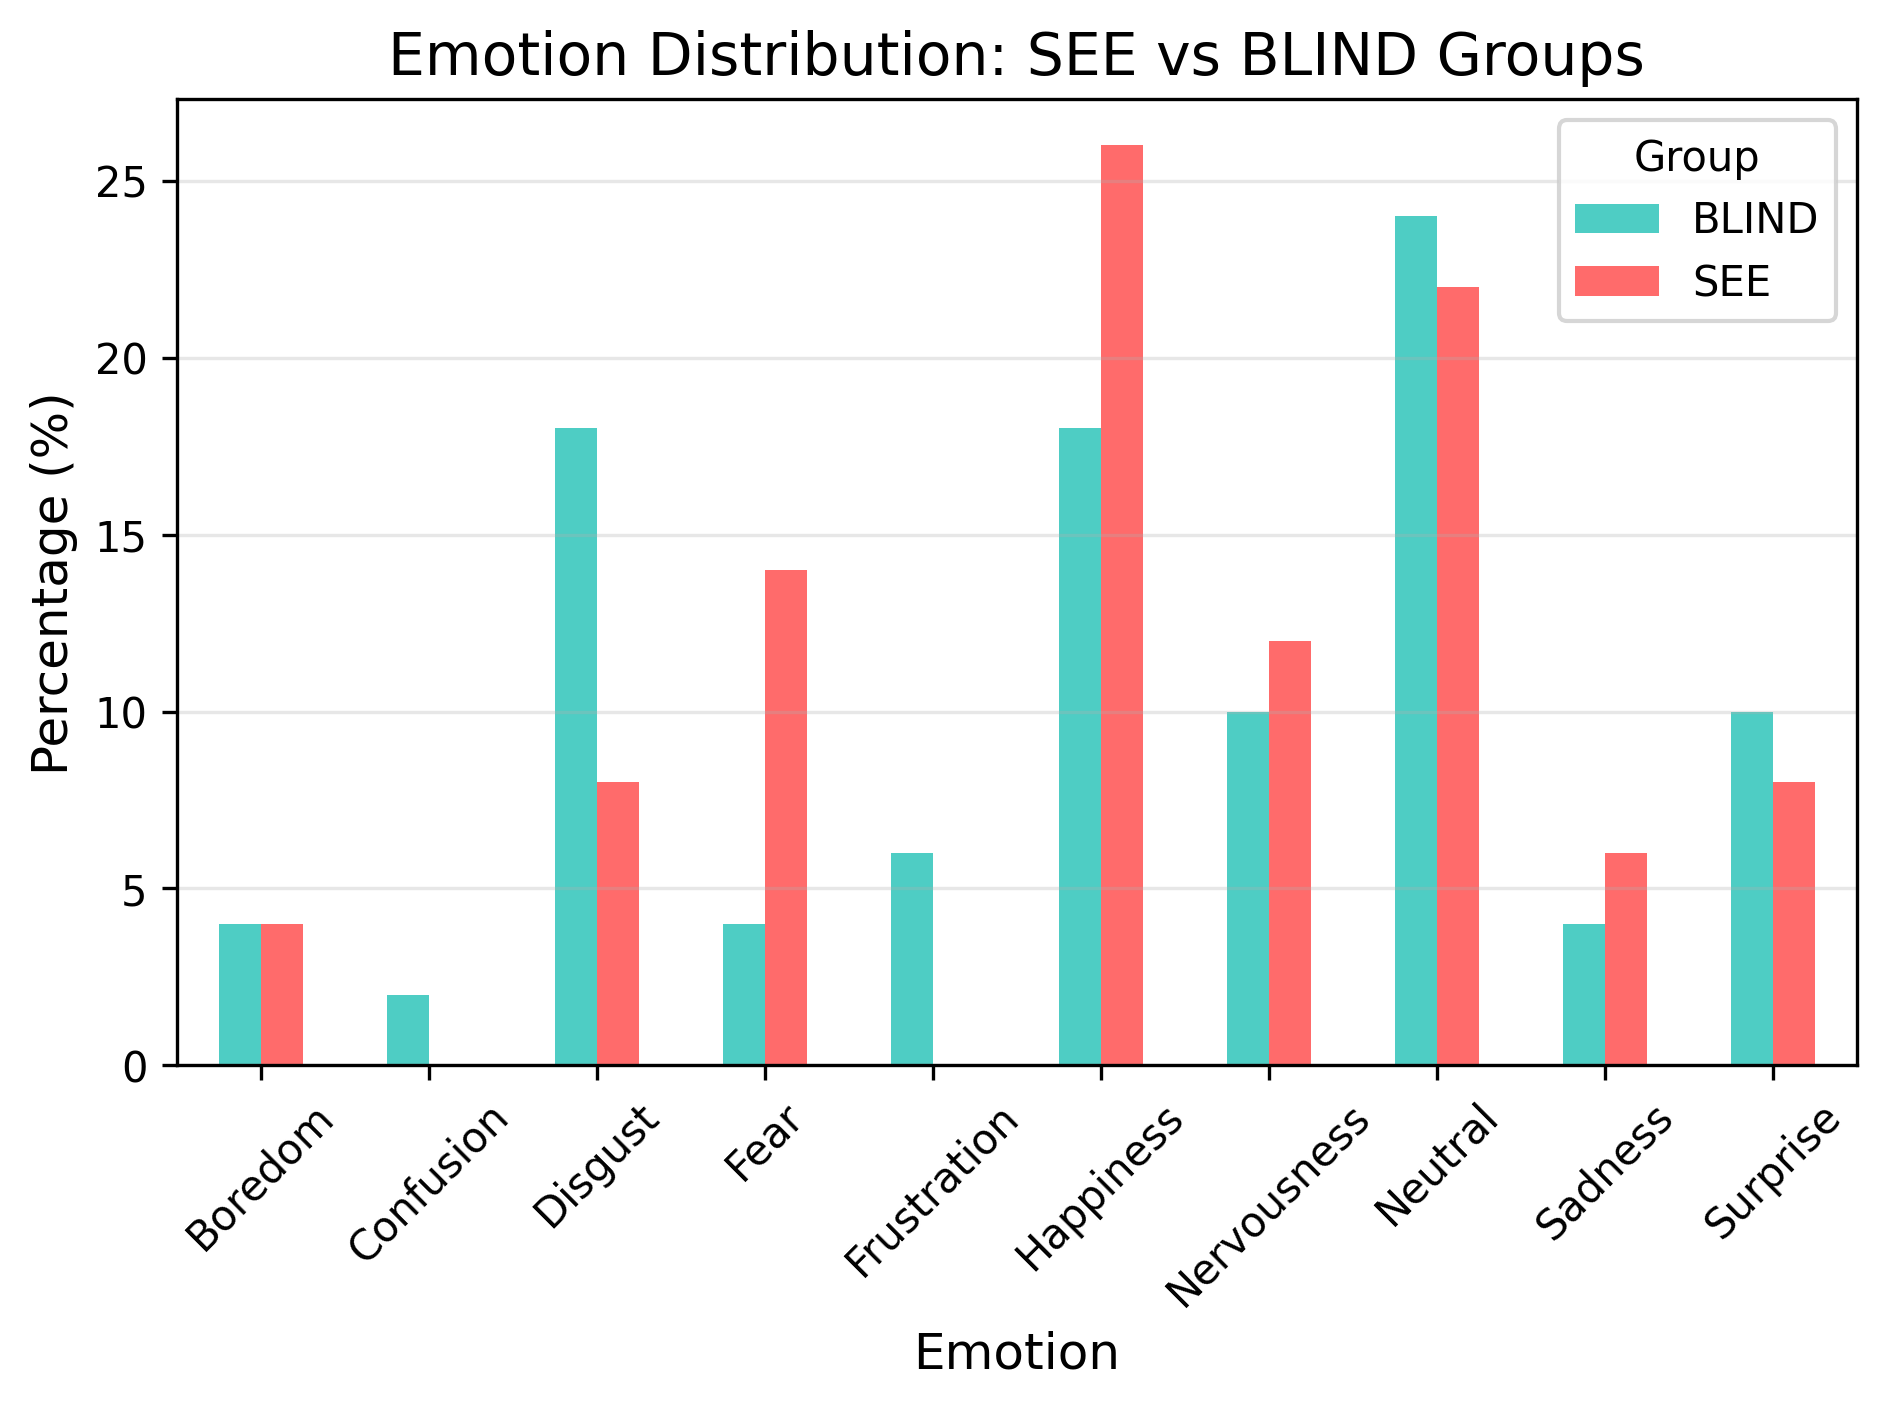
\includegraphics[width=\columnwidth]{group_emotion_analysis.png}
    \caption{Distribution of self-reported emotions by experimental group.}
    \label{fig:emotion-dist}
\end{figure}

\subsection{Statistical Analysis of Object Differences}

To test \textbf{Hypothesis 1}, we compared grasping frequency between objects using the Kruskal-Wallis H test due to non-normal data distribution. The test showed a statistically significant difference in grasping frequency between the five objects ($H(4) = 30.3$, $p < 0.001$). Post-hoc comparisons using Dunn's test with Bonferroni correction indicated that the grasping frequency for the spider ($M=18.09$) was significantly higher than for the donut ($M=7.02$, $p < 0.01$) and the pig ($M=9.48$, $p < 0.05$). No other pairwise differences reached significance.

The ranking order was: Spider (18.09) $>$ Toy (15.24) $>$ Box (10.28) $>$ Pig (9.48) $>$ Donut (7.02) events/s.

These findings provide strong support for \textbf{Hypothesis 1}, demonstrating that different emotionally evocative objects produce significantly different hand movement patterns during grasping.

\subsection{Arousal-Based Kinematic Analysis}

To investigate \textbf{Hypothesis 2}, we categorized trials based on self-reported emotions into high-arousal (fear, disgust, surprise) and low-arousal (neutral, happiness, comfort) groups and compared both grasping frequency and maximum velocity.

A Mann-Whitney U test was conducted to compare the grasping frequency between high-arousal ($M=11.00$ events/s) and low-arousal ($M=12.48$ events/s) conditions. The results indicated that the difference was not statistically significant ($U = 921.0$, $p = 0.270$).

Similarly, the maximum hand velocity was compared between high-arousal ($M=2.74$ px/frame) and low-arousal ($M=2.98$ px/frame) conditions. This difference was also not statistically significant ($U = 963.5$, $p = 0.432$).

These findings do not support \textbf{Hypothesis 2}, as emotional arousal did not produce a statistically significant change in either the frequency or maximum velocity of grasping movements in our study (see Fig.~\ref{fig:arousal-comparison}).

\begin{figure}[H]
    \centering
    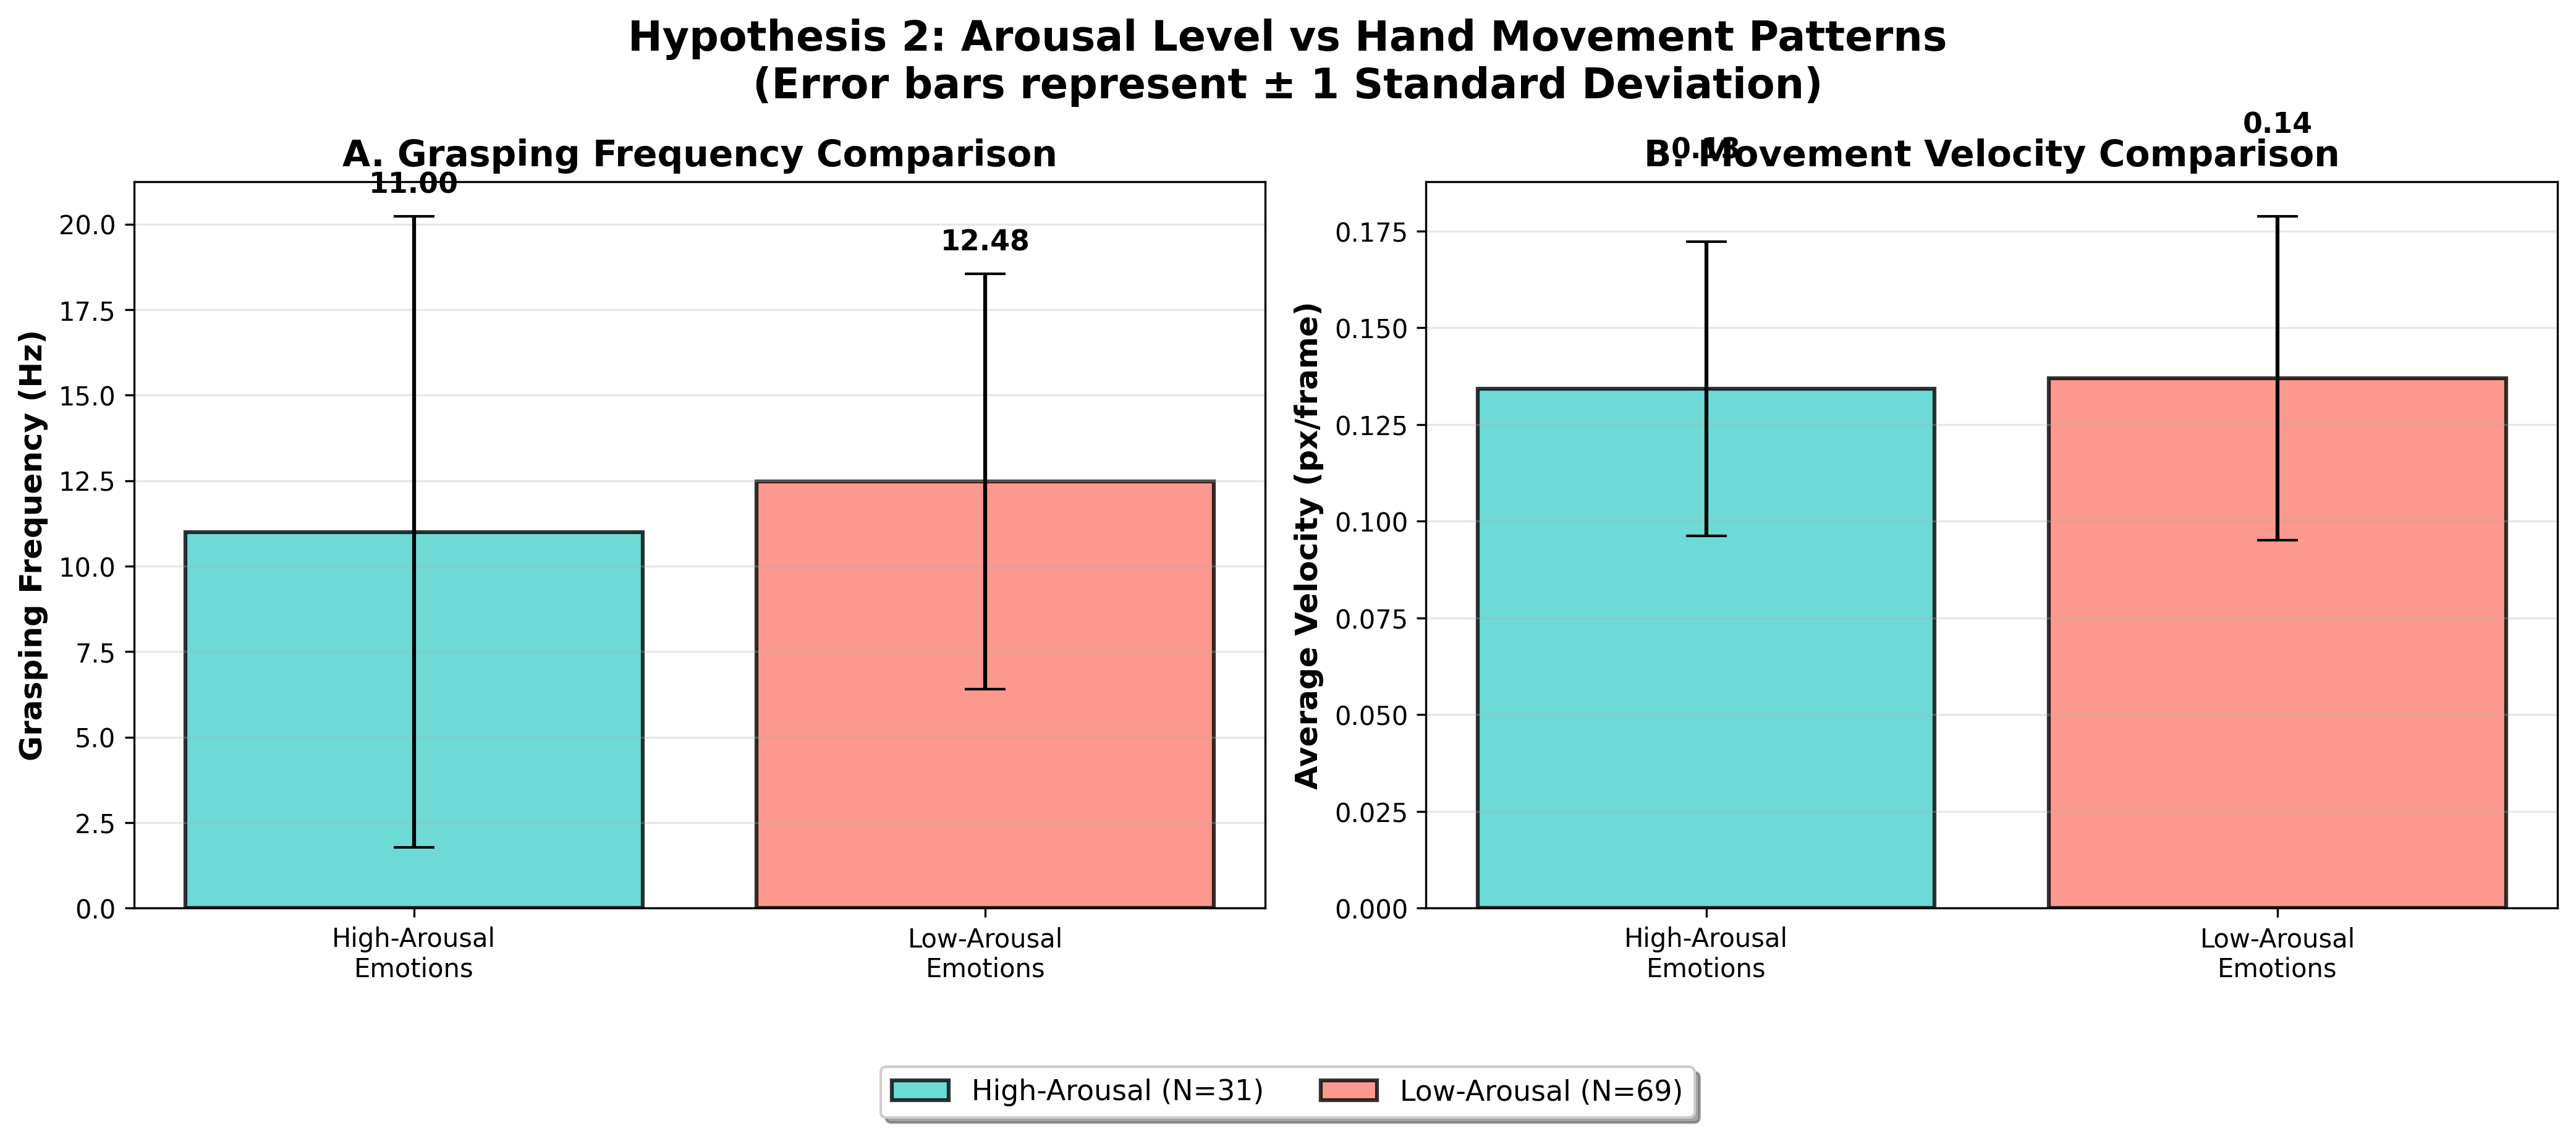
\includegraphics[width=\columnwidth]{figures/hypothesis2_arousal_comparison.png}
    \caption{Comparison of grasping frequency and maximum velocity between Low-Arousal and High-Arousal emotional conditions. Error bars represent the standard error of the mean (SEM). The p-values from Mann-Whitney U tests are shown above each comparison, indicating no statistically significant differences.}
    \label{fig:arousal-comparison}
\end{figure}

\subsection{Other Kinematic Measures}

No significant differences were found in other kinematic measures explored during the initial analysis, such as hand openness ratio or movement efficiency, across different objects or conditions (all $p > 0.1$).

\vfill\null
\columnbreak

% ------------------------------------------------------
\section{Discussion}
\label{sec:discussion}

\subsection{Hypothesis Validation}

Our findings provide mixed support for the proposed hypotheses. 
\textbf{Hypothesis 1} was strongly supported: different emotionally 
evocative objects produced markedly different hand movement patterns. 
The spider object generated the highest grasping frequency (18.09 events/s), 
while the donut showed the lowest activity (7.02 events/s), representing 
a 2.6-fold difference that aligns with the emotional intensity of these stimuli.

\textbf{Hypothesis 2}, which proposed that high-arousal emotions would lead to faster and more forceful movements, was \textbf{not supported} by our data. Our analysis found no statistically significant differences in either grasping frequency ($p=0.270$) or maximum hand velocity ($p=0.432$) between high-arousal and low-arousal conditions.

This null finding is a significant result in itself and prompts a deeper consideration of the emotion-motor interface. While some literature suggests arousal energizes motor activity, our results indicate this relationship may not be straightforward or universal. Several factors could contribute to this outcome. First, \textit{maximum velocity} might not be the most sensitive metric; temporal dynamics such as acceleration or the time to peak velocity could be more telling. Second, the broad categorization of "high-arousal" emotions may mask opposing effects; for example, the high-arousal state of fear (spider) might promote rapid movement, while the high-arousal state of disgust (donut) could promote freezing or withdrawal, with these effects cancelling each other out in a combined analysis. This suggests that future research should focus on emotion-specific motor signatures rather than relying on broad dimensions like arousal alone.

\subsection{Emotion-Specific Motor Patterns}

Despite the lack of an overall arousal effect, the distinct kinematic signatures for each object (as shown in our test of Hypothesis 1) reveal how emotional content shapes motor behavior~\cite{emotion_motor2021}. Fear-inducing stimuli (spider) elicited 
rapid, frequent grasping movements, potentially reflecting defensive or 
exploratory responses to threat. Conversely, disgust-evoking objects (donut) 
produced minimal contact, consistent with avoidance behaviors. Neutral 
objects (box, toy) showed intermediate patterns, while the comfort object 
(pig) generated moderate but sustained interaction.

These findings extend beyond simple arousal effects, suggesting that 
specific emotions activate distinct motor programs~\cite{embodied_emotion2022}. The spider's high 
activity may reflect evolutionary preparedness for threat detection, 
while disgust-related avoidance serves protective functions against 
contamination.

\subsection{Visual vs. Non-Visual Processing}

Contrary to expectations, visual preview did not significantly affect 
overall grasping behavior. The non-significant group difference 
($p = 0.791$) suggests that tactile-emotional responses may be as 
robust as visual-emotional responses in driving motor behavior. This 
finding has important implications for understanding multisensory 
emotion processing and supports the role of haptic perception in 
emotional evaluation.

The greater variability in the \textsc{Non-Visual} condition may reflect 
individual differences in tactile sensitivity or emotional processing 
when visual cues are absent. This variability could be leveraged in 
future studies to examine individual differences in emotion-motor coupling.

\subsection{Methodological Insights}

Our smartphone-based motion tracking approach successfully captured 
emotionally relevant motor variations, demonstrating the viability of 
accessible technology for behavioral research. The three-category 
movement classification (grasping, holding, other) effectively 
differentiated object-specific interaction patterns.

The alignment between intended emotional categories and participant 
responses validates our object selection strategy. However, the 
predominance of neutral responses (47\% of reports) suggests that 
naturalistic settings may attenuate emotional responses compared to 
laboratory paradigms.

\subsection{Applications and Implications}

\textbf{Human-Computer Interaction:} Real-time analysis of hand 
kinematics could enable emotion-aware interfaces that adapt to user 
affective states during object manipulation tasks.

\textbf{Clinical Applications:} Non-invasive kinematic assessment 
may complement traditional emotional evaluation methods, particularly 
for populations with communication difficulties.

\textbf{Affective Computing:} The emotion-specific motor signatures 
identified here could inform machine learning models for automatic 
emotion recognition in human-robot interaction scenarios.

\subsection{Limitations and Future Directions}

Several limitations constrain interpretation. The sample size (n=20) 
limits statistical power for detecting subtle effects. The naturalistic 
setting, while ecologically valid, reduced experimental control over 
confounding variables. Future studies should incorporate physiological 
measures (heart rate, skin conductance) to validate emotional arousal 
independent of self-report.

The video analysis methodology, while accessible, lacks the precision 
of specialized motion capture systems. Direct force measurement would 
provide additional insights into grip strength variations. Longitudinal 
designs could examine whether emotion-motor coupling patterns remain 
stable across sessions or show habituation effects.

Future work should explore individual differences in emotion-motor 
coupling, investigate developmental aspects of this relationship, and 
examine how cultural background influences emotional responses to objects.

% ------------------------------------------------------
\section{Conclusion}
\label{sec:conclusion}

This study demonstrates that emotional responses to objects systematically 
influence hand movement patterns during grasping tasks. Using accessible 
smartphone-based motion tracking, we identified distinct kinematic signatures 
for objects evoking different emotions, with fear-inducing stimuli generating 
the highest motor activity and disgust-evoking objects producing avoidance 
behaviors.

Our findings contribute to understanding emotion-motor coupling in several ways. 
First, we provide evidence that object-specific emotional responses translate 
into measurable kinematic differences, supporting theories of embodied emotion. 
Second, we show that emotional valence and approach-avoidance tendencies may 
be more predictive of motor behavior than arousal level alone. Third, we 
demonstrate that tactile-emotional processing can drive motor responses as 
effectively as visual-emotional processing.

The practical implications extend to human-computer interaction, clinical 
assessment, and affective computing applications. Real-time kinematic analysis 
could enable emotion-aware technologies that respond to users' affective states 
through their natural hand movements. For clinical populations with limited 
verbal communication, kinematic assessment offers a non-invasive window into 
emotional processing.

Future research should address the limitations identified here through larger 
samples, physiological validation, and examination of individual differences. 
The integration of emotion and motor control revealed in this work opens new 
avenues for understanding how feelings shape actions in human behavior.

% ------------------------------------------------------
\section*{References}

Please number citations consecutively within brackets \cite{b1}. The 
sentence punctuation follows the bracket \cite{b2}. Refer simply to the reference 
number, as in \cite{b3}---do not use ``

\begin{thebibliography}{00}

\bibitem{b1} 
S. J. Lederman and R. L. Klatzky, 
``Hand movements: A window into haptic object recognition,'' 
\textit{Cognitive Psychology}, vol. 19, no. 3, pp. 342--368, 1987.

\bibitem{b2} 
P. O. Esteves, L. A. S. Oliveira, A. A. Nogueira-Campos, G. Saunier, T. Pozzo, J. M. Oliveira, E. C. Rodrigues, E. Volchan, and C. D. Vargas, 
``Motor planning of goal-directed action is tuned by the emotional valence of the stimulus: A kinematic study,'' 
\textit{Scientific Reports}, vol. 6, Article no. 28780, 2016.

\bibitem{mediapipe2019} 
C. Lugaresi et al., 
``MediaPipe: A framework for building perception pipelines,'' 
arXiv preprint arXiv:1906.08172, 2019. 
[Online]. Available: https://arxiv.org/abs/1906.08172

\bibitem{opencv2015}
G. Bradski and A. Kaehler,
``Learning OpenCV 3: Computer Vision in C++ with the OpenCV Library,''
O'Reilly Media, Inc., 2015.

\bibitem{cohen1988}
J. Cohen,
\textit{Statistical Power Analysis for the Behavioral Sciences}, 2nd ed.
Hillsdale, NJ: Lawrence Erlbaum Associates, 1988.

\bibitem{emotion_motor2021}
A. Cavallo et al.,
``Emotion-specific motor patterns during action observation,''
\textit{Emotion}, vol. 21, no. 7, pp. 1515--1525, 2021.

\bibitem{affective_haptics2023}
H. Culbertson, S. B. Schorr, and A. M. Okamura,
``Haptics: The present and future of artificial touch sensation,''
\textit{Annual Review of Control, Robotics, and Autonomous Systems}, vol. 6, pp. 385--409, 2023.

\bibitem{embodied_emotion2022}
P. Winkielman, P. Niedenthal, J. Wielgosz, J. Eelen, and L. C. Kavanagh,
``Embodiment of cognition and emotion,''
in \textit{APA Handbook of Personality and Social Psychology}, 
American Psychological Association, 2022, pp. 151--175.

\end{thebibliography}

\end{document}